% !TEX TS-program = pdflatex
% !TEX encoding = UTF-8 Unicode

% This is a simple template for a LaTeX document using the "article" class.
% See "book", "report", "letter" for other types of document.

\documentclass[11pt]{article} % use larger type; default would be 10pt

\usepackage[utf8]{inputenc} % set input encoding (not needed with XeLaTeX)

%%% Examples of Article customizations
% These packages are optional, depending whether you want the features they provide.
% See the LaTeX Companion or other references for full information.

%%% PAGE DIMENSIONS
\usepackage{geometry} % to change the page dimensions
\geometry{a4paper} % or letterpaper (US) or a5paper or....
\geometry{margin=1.9cm}
% \geometry{margin=2in} % for example, change the margins to 2 inches all round
% \geometry{landscape} % set up the page for landscape
%   read geometry.pdf for detailed page layout information

\usepackage{graphicx} % support the \includegraphics command and options

% \usepackage[parfill]{parskip} % Activate to begin paragraphs with an empty line rather than an indent

%%% PACKAGES
\usepackage{booktabs} % for much better looking tables
\usepackage{array} % for better arrays (eg matrices) in maths
\usepackage{paralist} % very flexible & customisable lists (eg. enumerate/itemize, etc.)
\usepackage{verbatim} % adds environment for commenting out blocks of text & for better verbatim
\usepackage{subfig} % make it possible to include more than one captioned figure/table in a single float
% These packages are all incorporated in the memoir class to one degree or another...

%%% HEADERS & FOOTERS
\usepackage{fancyhdr} % This should be set AFTER setting up the page geometry
\pagestyle{fancy} % options: empty , plain , fancy
\renewcommand{\headrulewidth}{0pt} % customise the layout...
\lhead{}\chead{}\rhead{}
\lfoot{}\cfoot{\thepage}\rfoot{}

%%% SECTION TITLE APPEARANCE
\usepackage{sectsty}
\allsectionsfont{\sffamily\mdseries\upshape} % (See the fntguide.pdf for font help)
% (This matches ConTeXt defaults)

%%% ToC (table of contents) APPEARANCE
\usepackage[nottoc,notlof,notlot]{tocbibind} % Put the bibliography in the ToC
\usepackage[titles,subfigure]{tocloft} % Alter the style of the Table of Contents
\renewcommand{\cftsecfont}{\rmfamily\mdseries\upshape}
\renewcommand{\cftsecpagefont}{\rmfamily\mdseries\upshape} % No bold!

\usepackage[lined,boxed,commentsnumbered]{algorithm2e}
\usepackage{amsmath}
%%% END Article customizations

%%% The "real" document content comes below...

\title{Homework 2}
\author{Jiachi Liu}
%\date{} % Activate to display a given date or no date (if empty),
         % otherwise the current date is printed 

\begin{document}
\maketitle

\section{Decision Tree}
Let $D$ be the training set.\\
Attributes:\\
$color = \{yellow,green\}$
$size = \{small,large\}$
$shape = \{round,irregular\}$\\
Class Label:\\
$edible=\{+,-\}$

\begin{enumerate}
\item Create root node $N$ for tuples in  $D$.
\item To find the splitting criterion for those tuples, compute the information gain of each attribute.\\
$info(D) = -\frac{9}{16}log(\frac{9}{16})-\frac{7}{16}log(\frac{7}{16})=0.989$\\
$info_{color}(D) = \frac{3}{16}*[-\frac{1}{3}log(\frac{1}{3})-\frac{2}{3}log({\frac{2}{3}})] +
 				\frac{13}{16}*[-\frac{8}{13}log(\frac{8}{13})-\frac{5}{13}log({\frac{5}{13}})] =0.953$\\
$gain(color)=0.989 - 0.953 = 0.036$\\
$info_{size}(D)=\frac{8}{16}*[-\frac{6}{8}log(\frac{6}{8})-\frac{2}{8}log(\frac{2}{8})] +
			 \frac{8}{16}*[-\frac{3}{8}log(\frac{3}{8})-\frac{5}{8}log(\frac{5}{8})] = 0.883 $\\
$gain(size)=0.989-0.883=0.106$\\
$info_{shape} = \frac{12}{16}*[-\frac{6}{12}log(\frac{6}{12})-\frac{6}{12}log(\frac{6}{12})]+
			\frac{4}{16}*[-\frac{3}{4}log(\frac{3}{4})-\frac{1}{4}log(\frac{1}{4})] = 0.953$\\
$gain(shape) = 0.989-0.953=0.036$\\
% Check from here!!!%
Since $size$ has the greatest information gain, select it as splitting attribute and label N with $size$. And $D$ is splitted into two subsets $D_1$, which contains tuples that have `small' in $size$ and $D_2$ which contains tuples have `large' in $size$.
\item Create node $N_1$ for tuples in $D_1$.
\item Compute the splitting criterion for those tuples, which $size=small$.\\
$info(D_1)=-\frac{6}{8}log(\frac{6}{8})-\frac{2}{8}log(\frac{2}{8})=0.811$\\
$info_{color}(D_1)=\frac{2}{8}*[-\frac{1}{2}log(\frac{1}{2})-\frac{1}{2}log(\frac{1}{2})]+
				\frac{6}{8}*[-\frac{5}{6}log(\frac{5}{6})-\frac{1}{6}log{\frac{1}{6}}]=0.738$\\
$gain(color) = 0.811-0.738=0.073$\\
$info_{shape}(D_1)=\frac{6}{8}*[-\frac{4}{6}log(\frac{4}{6})-\frac{2}{6}log(\frac{2}{6})]+
				\frac{2}{8}*[-\frac{2}{2}log(\frac{2}{2})]=0.689$\\
$gain(shape) = 0.811 - 0.689 = 0.122$\\
Choose $shape$ as the label of $N_1$. Split $D_1$ into $D_3$ and $D_4$ where $D_3$ is $shape = round$ and $D_4$ is $shape=irregular$.
\item For $D_3$, there is only one attribute in it so create a new node $N_3$ labeled as $color$. Split $D_3$ into two subset where color=green or color=yellow. For color=yellow, the majority class is '+', created a node labeled '+'. For color=green, create node and labeled '-' since it is the major class.
\item For $D_4$, for both color=yellow or color=green the class is '+'. Thus create a node labeled as '+'.
\item Do the above steps again on $D_2$.\\
$info(D_2)=-\frac{3}{8}log(\frac{3}{8})-\frac{5}{8}log(\frac{5}{8})=0.954$\\
$info_{color}(D_2) = \frac{1}{8}*[-\frac{1}{1}log(\frac{1}{1})]+
				\frac{7}{8}*[-\frac{3}{7}log(\frac{3}{7})-\frac{4}{7}log(\frac{4}{7})]=0.862$\\
$gain(color) = 0.954-0.862=0.092$\\
$info_{shape}(D_2) = \frac{2}{8}*[-\frac{1}{2}log(\frac{1}{2})-\frac{1}{2}log(\frac{1}{2})]+
				\frac{6}{8}*[-\frac{2}{6}log(\frac{2}{6})-\frac{4}{6}log(\frac{4}{6})]=0.939$\\
$gain(shape) = 0.954-0.939 = 0.015$\\
Create a node labeled as $color$. Split $D_2$ into $(color=yellow)$ and $(color=green)$.
\item For color=yellow, create a node labeled as $shape$ and split into $ (shape=round)$ and $(shape=irregular)$. Create leaf node `-' for shape is round and leaf node '+' for shape = irregular.
\item For color=green, create a node labeled as $shape$ and split into $(shape=round)$ and $(shape=irregular)$. Create leaf node `+' for $shape=round$ since it is empty attach majority class in $D$. Create leaf `-' for $(shape=irregular)$.
\end{enumerate}
\begin{figure}[htbp]
\begin{center}
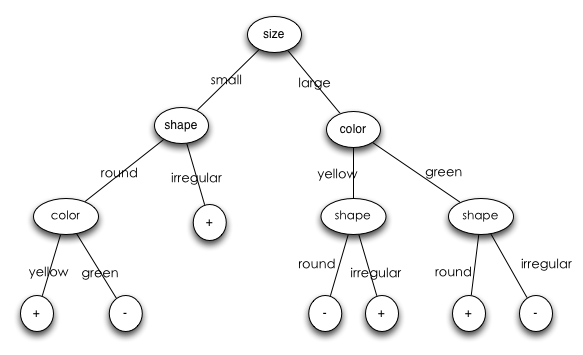
\includegraphics[width=400px]{dt.png}
\caption{Decision Tree}
\label{default}
\end{center}
\end{figure}

\section{Support Vector Machine}
\subsection{Question 1}
Let $x_i \in X$ where $X$ is the set of all tuples and $1\leq i \leq 20$. According to the values of $\alpha_i$, $x_7$, $x_8$ and $x_{20}$ is the support vector.
\subsection{Question 2}
$w = \sum {\alpha_i  y_i  x_i} = 0.4952*1*[0.53,0.77] + 0.0459*(-1)*[2.05,-0.62]+0.4493*(-1)*[1.63,-0.91]=[-0.563998,0.818625]$
\subsection{Question 3}
$b =\frac{ (1-[-0.563998,0.818625][0.53,0.77])+(-1-[-0.563998,0.818625][2.05,-0.62])+(-1-[-0.563998,0.818625][1.63,-0.91])}{3}
=0.66552886$
\subsection{Question 4}
$f(x) = -0.563998x_1+0.818625x_2+0.66552886$
\subsection{Question 5}
$x=(-1,2)$\\
$f(x) = -0.563998*(-1)+0.818625*2+0.66552886=1$\\
Class label of $x$ is 1.

\section{Clustering for Matrix Data}
\subsection{List four limitations of K-means, and name one algorithm for each limitation that can overcome that limitation}
\begin{enumerate}
\item Applicable only to objects in a continuous n-dimensional space. Using K-mode to categorial data.
\item Need to specify k. Using AGNES algorithm
\item Sensitive to noisy data and outliers. Using PAM algorithm to replace the mean value of objects in cluster with most centrally located object in a cluster.
\item Not suitable to discover clusters with non-convex shapes. Using DBSCAN.
\end{enumerate}

\subsection{Clustering Evaluation}
Majority class and members of the majority class in each cluster is:\\
$c_1=[3,3,3,3,3,1]$\\
$c_2=[2,2,2,2,2,4]$\\
$c_3=[1,1,1,4,1]$\\
$c_4=[4,4,4]$\\
$purity = \frac{1}{20}*(5+5+4+3)=0.85$\\
$TP+FP = \binom{6}{2} + \binom{6}{2} + \binom{5}{2} + \binom{3}{2} = 43$\\
$TP = \binom{5}{2} + \binom{5}{2} +\binom{4}{2} +\binom{3}{2} = 29$\\
$FP = 43-29=14$\\
$FN+TN = 6*(6+5+3) + 6*(5+3) + 5*3 = 147$\\
$FN = 4+ 3 + 4 = 11$\\
$TN = 147 - 11 = 136$\\
$P = TP/(TP+FP) = 29/43 = 0.6744$\\
$R = TP/(TP+FN) = 29/(29+11) = 0.725$\\
$F-measure = P*R/(P+R) = 0.3494$
\begin{table}[htdp]
\caption{Confusion Matrix}
\begin{center}
\begin{tabular}{|c|c|c|}
\hline
& same cluster & different clusters \\
\hline
Same class & TP = 29 & FN = 11\\
\hline
Different classes & FP = 14 & TN =136\\
\hline
\end{tabular}
\end{center}
\label{default}
\end{table}%
\\For normalized mutual information:\\
$I = \frac{1}{20}log(\frac{20}{6*5}) +\frac{5}{20}log(\frac{20*5}{6*5})
	+\frac{1}{20}log(\frac{20}{6*5}) +\frac{5}{20}log(\frac{20*5}{6*5})
	+\frac{1}{20}log(\frac{20}{5*5}) +\frac{4}{20}log(\frac{20*4}{5*5})
	+\frac{3}{20}log(\frac{20*3}{3*5})=1.4295$
$H(C) = -\frac{6}{20}log(\frac{6}{20})-\frac{6}{20}log(\frac{6}{20})-\frac{5}{20}log(\frac{5}{20})-\frac{3}{20}log(\frac{3}{20}) = 1.9527$\\
$H(\Omega) = -4*\frac{5}{20}log(\frac{5}{20})= 2$\\
$NMI = 1.4295/\sqrt{1.9527*2} = 0.723$\\

\section{Frequent Pattern Mining for Set Data}
\subsection{Aprior}
sup\_min = 60\%, sup\_min\_count = 5*60\% = 3\\
Using Aprior Algorithm as the following:\\
$c_1=[M:3,O:3,N:2,K:5,E:4,Y:3,D:1,A:1,U:1,C:2,I:1]$\\
$L_1=[M:3,O:3,K:5,E:4,Y:3]$\\
$c_2=[MO:1,MN:1,MK:3,ME:2,MY:2,ON:2,OK:3,OE:3,OY:2,NK:2,NE:2,NY:2,KE:4,KY:3,EY:2]$\\
$L_2=[MK:3,OK:3,OE:3,KE:4,KY:3]$\\
$c_3=[OKE:3,KEY:2]$\\
$L_3=[OKE:3]$\\
Joint $L_3$ with itself which will not produce new itemset. Thus stop. The frequent itemset is \{OKE, MK,OK,OE,KE,KY,M,O,K,E,Y\}. Create the associate rules for OKE:\\
$O -> KE$ $confidence= 3/3 = 100\%$\\
$K -> OE$ $confidence= 3/5 = 60\%$\\
$E -> OK$ $confidence= 3/4 = 75\%$\\
$KE -> O$ $confidence= 3/4 = 75\%$\\
$OE -> K$ $confidence= 3/3 = 100\%$\\
$OK -> E$ $confidence= 3/3 = 100\%$\\
The rules that matching the given metarules is $OE -> K$ and $OK -> E$.
\subsection{FP-Growth}
$F-list = [K:5,E:4,M:3,O:3,Y:3]$
\begin{figure}[htbp]
\begin{center}
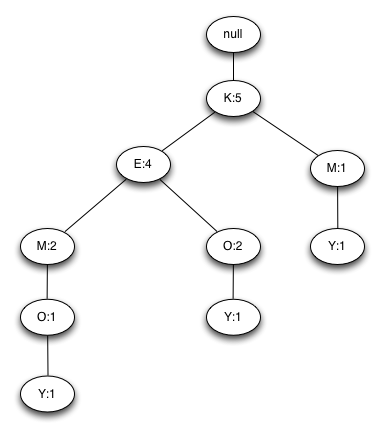
\includegraphics[width=300px]{fptree.png}
\caption{FP-Tree}
\label{default}
\end{center}
\end{figure}

\begin{table}[htdp]
\caption{Mining the FP-Tree by Creating Conditional (Sub-)Pattern Bases}
\begin{tabular}{|c|c|c|c|}
item & Conditional Pattern Base & Conditional FP-tree & Frequent Patterns Generated\\
Y & $\{KEMO:1\}\{KEO:1\}\{KM:1\}$ & $<K:3>$ & \{K,Y:3\}\\
O & $\{KEM:1\}\{KE:2\}$ & $<K:3, E:3>$ & \{K,O:3\}\{E,O:3\}\{K,E,O:3\}\\
M & $\{KE:2\}\{K:1\}$ & $<K:3>$ & \{K,M:3\}\\
E & $\{K:4\}$ & $<K:4>$ & \{K,E:4\}\\
\end{tabular}
\label{default}
\end{table}
Thus all frequent itemsets is \{KEO,KY,KO,EO,KM,KE,M,O,K,E,Y\}. Create Associate rules for OKE:\\
$O -> KE$ $confidence= 3/3 = 100\%$\\
$K -> OE$ $confidence= 3/5 = 60\%$\\
$E -> OK$ $confidence= 3/4 = 75\%$\\
$KE -> O$ $confidence= 3/4 = 75\%$\\
$OE -> K$ $confidence= 3/3 = 100\%$\\
$OK -> E$ $confidence= 3/3 = 100\%$\\
The rules that matching the given metarules is $OE -> K$ and $OK -> E$.
\subsection{Summary}
The FP-growth algorithm is more efficient than Apriori Algorithm. For Apriori, it has two costly procedures. First it may need to generate a huge number of candidate sets if we have many frequent 1-itemset. Secondly, It may need to repeatedly scan the whole database and check a large set of candidates by pattern matching. To solve these two problems, FP-growth adopts a divide-and-conquer strategy to find all frequent itemsets.
\end{document}